\documentclass[11pt]{article}

\usepackage[margin=1in]{geometry}
\usepackage{amsmath,amssymb}
\usepackage{graphicx}
\usepackage{booktabs}
\usepackage{siunitx}
\usepackage[round]{natbib}
\usepackage[colorlinks=true,linkcolor=blue,citecolor=blue,urlcolor=blue]{hyperref}
\usepackage{cleveref}

\graphicspath{{figures/}}

\newcommand{\pd}[2]{\frac{\partial #1}{\partial #2}}
\newcommand{\mdot}{\dot{m}}

\title{A Godunov-Type Finite-Volume Model for the Transient Blowdown of a
Pressurized Vertical Well:\\ Formulation, Verification, and Baseline
Nitrogen Results}

\author{Jader R. Barbosa, Jr.\thanks{Craft \& Hawkins Department of
Petroleum Engineering, Louisiana State University, Baton Rouge, LA.}}

\date{\today\\[1ex]\small Working document --- Phase 3, Stage 1 of the
HyperCO$_2$ framework}

\begin{document}
\maketitle

\begin{abstract}
This document describes the formulation, numerical implementation, and
verification of a one-dimensional transient compressible-flow model for the
blowdown of a pressurized vertical well through a wellhead restriction. The
governing mass, momentum, and total-energy equations are solved in
conservative form with a Godunov-type finite-volume method employing
MUSCL--Hancock reconstruction and the HLLC approximate Riemann solver, a
numerical architecture selected on the basis of systematic shock-tube
benchmarks against the split-coefficient-matrix method (SCMM) used in
earlier work \citep{gessner2010}. Gravity, wall friction, and fluid--wall
heat transfer enter as source terms; the gravitational work term is
discretized in an energy-consistent face-flux form that closes the discrete
total-plus-potential energy budget to machine precision. The wellhead is
modeled as a choke coupled to the interior solution through the outgoing
characteristic, yielding a physically consistent choked/unchoked/closed
discharge sequence. Verification comprises exact shock-tube solutions,
conservation audits, the quasi-static lumped-vessel limit, and grid,
time-step, and boundary-condition sensitivity studies. Baseline results are
presented for the adiabatic blowdown of a \SI{2000}{ft} nitrogen-filled
well from \SI{13.79}{\mega\pascal}. The thermodynamic-property model is
isolated behind an interface so that real-fluid CO$_2$ properties can
replace the ideal-gas closure without modification of the flow solver.
\end{abstract}

%=============================================================
\section{Introduction}
%=============================================================

Transient depressurization (blowdown) of wells and pipelines containing
compressed gas is a canonical problem in well control, CO$_2$ transport and
storage operations, and the repurposing of oil and gas wells for energy
storage. The rapid opening of a wellhead valve launches an expansion wave
into the wellbore, followed by a long quasi-static discharge during which
the contained fluid cools substantially by expansion work. For CO$_2$, the
associated temperature excursions can cross the saturation locus, with
consequences for well integrity and metering; a predictive transient model
is therefore a prerequisite for the design and interpretation of blowdown
and injection tests.

The present work is the third phase of a numerical framework whose starting
point was the Fortran implementation of the split coefficient matrix method
(SCMM) developed in \citet{gessner2010} following
\citet{chakravarthy1980} and \citet{stadtke2006}, with linear systems
solved by the banded routine of \citet{aziz1979}. In Phases~1--2 the
original single-phase SCMM solvers (conservative and non-conservative
formulations, first- and second-order upwind variants) were reconstructed
in Python and validated against exact shock-tube solutions, reproducing the
original error tables; Godunov-type finite-volume (FV) alternatives were
then evaluated on identical benchmarks. The FV method with MUSCL--Hancock
reconstruction \citep{vanleer1984,toro2009} and the HLLC approximate
Riemann solver \citep{toro1994} proved approximately one order of magnitude
more accurate than the best original scheme at two orders of magnitude
lower computational cost, with exact discrete conservation --- properties
the quasi-linear SCMM discretization cannot provide. That evidence, rather
than a priori preference, fixed the architecture adopted here.

This document records (i)~the mathematical model and its source terms,
(ii)~the numerical method, including the wellhead choke boundary condition
and an energy-consistent treatment of gravitational work, (iii)~the
verification campaign, and (iv)~baseline results for adiabatic nitrogen
blowdown of a \SI{2000}{ft} well. Planned extensions --- real-fluid CO$_2$
thermodynamics, and conjugate heat transfer with the completion and
formation --- are outlined in \cref{sec:outlook}.

%=============================================================
\section{Problem formulation}
%=============================================================
\label{sec:problem}

A vertical well of depth $L = \SI{609.6}{m}$ (\SI{2000}{ft}) and constant
circular cross-section (inner diameter $D$, flow area $A = \pi D^2/4$) is
initially closed and filled with quiescent gas at uniform pressure $p_0$
and temperature $T_0$. The axial coordinate $z$ is measured upward from
the closed bottom ($z=0$) to the wellhead ($z=L$). At $t=0$ a choke of
bore diameter $d_c$ and discharge coefficient $C_d$ at the wellhead is
opened instantaneously to an external environment at back pressure $p_b$.
The baseline configuration is summarized in \cref{tab:baseline}.

\begin{table}[htb]
\centering
\caption{Baseline case definition.}
\label{tab:baseline}
\begin{tabular}{ll}
\toprule
Fluid & N$_2$, ideal gas ($R=\SI{296.8}{J/(kg.K)}$, $\gamma=1.40$)\\
Well depth $L$ & \SI{609.6}{m} (\SI{2000}{ft})\\
Well inner diameter $D$ & \SI{0.100}{m}\\
Initial state & uniform, $p_0=\SI{13.79}{\mega\pascal}$ (\SI{2000}{psi}), $T_0=\SI{300}{K}$, $u=0$\\
Choke & $d_c = \SI{12.7}{mm}$, $C_d = 0.84$, $p_b = \SI{101.325}{\kilo\pascal}$\\
Bottom boundary & closed (solid wall)\\
Walls & adiabatic (baseline); friction neglected (baseline)\\
\bottomrule
\end{tabular}
\end{table}

The quantities of interest are the axial--temporal fields $p(z,t)$,
$T(z,t)$, $\rho(z,t)$, $u(z,t)$, the wellhead mass flow rate $\mdot(t)$,
and the mass inventory $M(t)$.

%=============================================================
\section{Mathematical model}
%=============================================================
\label{sec:model}

\subsection{Governing equations}

One-dimensional transient compressible flow along the well axis is
governed by the conservation of mass, momentum, and total energy,
\begin{align}
\pd{\rho}{t} + \pd{(\rho u)}{z} &= 0, \label{eq:mass}\\
\pd{(\rho u)}{t} + \pd{}{z}\!\left(\rho u^{2} + p\right) &=
  -\rho g \;-\; \frac{f_D\,\rho\,u\,|u|}{2D}, \label{eq:mom}\\
\pd{E}{t} + \pd{}{z}\!\left[u\left(E + p\right)\right] &=
  -\rho u g \;+\; \frac{4\,q_w''}{D}, \label{eq:energy}
\end{align}
where $\rho$ is the density, $u$ the velocity (positive upward), $p$ the
pressure, $E = \rho\,(e + u^2/2)$ the total energy per unit volume, $e$
the specific internal energy, $g$ the gravitational acceleration, $f_D$
the Darcy friction factor, and $q_w''$ the wall heat flux into the fluid.
Wall shear appears only in the momentum equation: a stationary wall
performs no net work on the fluid, and frictional dissipation is recovered
automatically by the conservative total-energy formulation. The friction
factor, when enabled, is evaluated from the all-regime correlation of
\citet{churchill1977}.

\subsection{Equation of state}

The system is closed by an equation of state supplying
$(p, T, a) = f(\rho, e)$, where $a$ is the speed of sound. The solver and
the boundary conditions interact with the fluid exclusively through an
abstract property interface comprising this closure, the isentrope
$\rho(p;\,p_{\mathrm{ref}},\rho_{\mathrm{ref}})$, the outgoing-wave
(Riemann-invariant) velocity relation, and the isentropic-nozzle mass
flux. For the present stage the interface is implemented by a calorically
perfect gas,
\begin{equation}
p = \rho R T, \qquad e = c_v T, \qquad a = \sqrt{\gamma R T},
\end{equation}
with nitrogen properties; a real-fluid CO$_2$ implementation of the same
interface (evaluating the isentrope and invariant numerically) replaces
this class without modification of the flow solver.

\subsection{Thermal boundary hierarchy}

The wall heat flux $q_w''$ is supplied by an interchangeable thermal
model: (1)~adiabatic wall, $q_w''=0$ (baseline, this document);
(2)~prescribed wall temperature with convective coupling,
$q_w'' = h\,(T_w - T)$, $h$ from the Dittus--Boelter correlation
(simplified benchmark); (3)~prescribed or externally computed heat flux;
and (4)~the target formulation, conjugate coupling to transient radial
conduction through tubing, casing, cement, and formation, with
$q'' = -k_f\,(\partial T_f/\partial r)\big|_{r_w}$ at the wellbore wall.
Stages 3--4 are the subject of the next phase.

%=============================================================
\section{Numerical method}
%=============================================================
\label{sec:numerics}

\subsection{Finite-volume discretization}

Equations \eqref{eq:mass}--\eqref{eq:energy} are discretized on $N$
uniform cells of width $\Delta z = L/N$ in conservative finite-volume
form,
\begin{equation}
\mathbf{V}_j^{n+1} = \mathbf{V}_j^{n}
 - \frac{\Delta t}{\Delta z}\left(\mathbf{F}_{j+1/2} - \mathbf{F}_{j-1/2}\right)
 + \Delta t\, \mathbf{S}_j,
\qquad \mathbf{V} = \left[\rho,\; \rho u,\; E\right]^{T},
\end{equation}
with interface fluxes from the HLLC approximate Riemann solver
\citep{toro1994,toro2009} acting on MUSCL--Hancock-reconstructed primitive
variables (van~Leer limiter). The HLLC solver restores the contact wave
omitted by HLL, which is immaterial for the smooth blowdown interior but
retained for consistency with the shock-capturing benchmarks and for
robustness in later two-phase extensions. Time integration is explicit
under the CFL condition
$\Delta t = \mathrm{CFL}\,\Delta z / \max_j\left(|u_j| + a_j\right)$,
with $\mathrm{CFL} = 0.8$ unless stated otherwise.

\subsection{Source-term treatment}
\label{sec:sources}

Gravity is included in the Hancock predictor half-step (maintaining formal
second order), and the momentum source $-\rho g$, friction, and wall heat
flux are advanced with a Heun (trapezoidal) corrector. The gravitational
\emph{work} term in \cref{eq:energy} requires care: evaluating it as
$-\rho_j u_j g$ at cell centers leaves a residual in the discrete energy
budget that does \emph{not} converge with mesh or time-step refinement,
because the potential-energy inventory evolves according to the
\emph{face} mass fluxes while the work term samples cell-centered momenta.
The term is therefore discretized in the energy-consistent face-flux form
\begin{equation}
\left(-\rho u g\right)_j \;\longrightarrow\;
 -\,g\,\frac{F^{\rho}_{j-1/2} + F^{\rho}_{j+1/2}}{2},
\label{eq:gravwork}
\end{equation}
where $F^{\rho}$ denotes the time-centered HLLC mass flux. With
\cref{eq:gravwork} the discrete budget
\begin{equation}
\sum_j \left(E_j + \rho_j g z_j\right) A\,\Delta z
\;+\; \int_0^t \mdot\,\left(h_0 + gL\right)\,dt'
\;=\; \text{const}
\label{eq:budget}
\end{equation}
telescopes exactly (machine precision), where $h_0$ is the stagnation
enthalpy of the effluent. The scheme is not well-balanced in the sense of
preserving discrete hydrostatic equilibria exactly; residual velocities of
order \SI{5}{cm/s} (200 cells) persist in a closed hydrostatic column,
which is negligible against blowdown velocities but should be revisited if
long-time post-blowdown equilibria become of interest.

\subsection{Bottom boundary}

The closed bottom is an exact solid wall: the wall-face left state is the
mirror image (in velocity) of the MUSCL-reconstructed interior right
state, for which the HLLC mass and energy fluxes vanish identically.

\subsection{Wellhead choke boundary condition}
\label{sec:choke}

The wellhead must not be treated as a fixed-pressure boundary while a
restriction separates the well from the environment. The pipe-side face
state $(\rho_f, u_f, p_f)$ at $z = L$ is instead required to satisfy,
simultaneously:
\begin{enumerate}
\item \emph{Coupling to the interior.} The face lies on the isentrope
through the adjacent interior state $(\rho_i, u_i, p_i)$ and on its
outgoing $C^{+}$ characteristic,
\begin{equation}
u_f = u_i + \frac{2}{\gamma - 1}\left(a_i - a_f\right),
\qquad
\rho_f = \rho_i \left(p_f/p_i\right)^{1/\gamma};
\label{eq:cplus}
\end{equation}
\item \emph{Valve mass balance.} The flow accepted by the choke, modeled
as a quasi-steady isentropic nozzle fed by the stagnation state
$(p_{0f}, T_{0f})$ of the face flow, equals the pipe efflux:
\begin{equation}
\rho_f u_f A = C_d A_t\, G\!\left(p_{0f}, T_{0f}, p_b\right),
\qquad A_t = \pi d_c^2/4,
\label{eq:valve}
\end{equation}
where $G$ is the standard compressible-orifice mass flux, which is choked
when $p_b/p_{0f} \le \left(2/(\gamma+1)\right)^{\gamma/(\gamma-1)}$ and
subcritical otherwise.
\end{enumerate}
Substitution of \cref{eq:cplus} into \cref{eq:valve} yields a scalar
equation for $p_f$, solved by Brent iteration on a bracket bounded below
by the \emph{sonic face pressure} --- the $C^{+}$ coupling forbids a
supersonic pipe exit; if the valve demands more than the sonic pipe
supply, the exit itself runs sonic, recovering the open-pipe choking limit
$A_t \to A$ --- and above by the pressure at which \cref{eq:cplus} brings
the face to rest. When the interior stagnation pressure falls below
$p_b$, the valve closes (check-valve clamp; backflow excluded). The
resulting face flux
$\left[\rho_f u_f,\; \rho_f u_f^2 + p_f,\; u_f (E_f + p_f)\right]$
replaces the HLLC flux at the top face, so the interior update and the
discharge remain mutually consistent through the entire
choked~$\to$~unchoked~$\to$~closed sequence as the well depressurizes, and
$\mdot(t) = \rho_f u_f A$ is obtained as part of the solution.

%=============================================================
\section{Verification}
%=============================================================
\label{sec:verification}

\subsection{Shock-capturing heritage}

The HLLC/MUSCL--Hancock kernel was verified in Phase~2 on the single-phase
shock tube of \citet{gessner2010} (air; \SI{500}{\kilo\pascal},
\SI{400}{K} / \SI{100}{\kilo\pascal}, \SI{300}{K}; 4001-point grid)
against the exact Riemann solution. \Cref{tab:shocktube} summarizes the
mean absolute errors: the first-order Godunov scheme already matches the
best legacy SCMM variant, and MUSCL--Hancock improves on it by an order of
magnitude at a small fraction of the cost, with discrete conservation to
machine precision. The HLLC flux is indistinguishable from the exact
Riemann flux on this problem.

\begin{table}[htb]
\centering
\caption{Single-phase shock-tube benchmark at $t=\SI{3}{ms}$: mean
absolute errors against the exact solution (4001 nodes / 4000 cells).
SCMM rows: Python reconstruction of \citet{gessner2010}; thesis values in
parentheses.}
\label{tab:shocktube}
\begin{tabular}{lccccc}
\toprule
Scheme & $p$ [\si{Pa}] & $u$ [\si{m/s}] & $\rho$ [\si{kg/m^3}] & $T$ [\si{K}] & Wall time [\si{s}]\\
\midrule
SCMM non-cons., 2nd order & 3027 (2713) & 4.29 & 0.0230 & 2.02 & 186\\
SCMM conservative, 2nd order & 383 (312) & 0.44 & 0.0041 & 0.35 & 399\\
FV first order, HLLC & 316 & 0.28 & 0.0041 & 0.41 & 1.4\\
FV MUSCL--Hancock, HLLC & 34.9 & 0.040 & 0.00057 & 0.065 & 2.0\\
\bottomrule
\end{tabular}
\end{table}

\subsection{Conservation audits}

For the closed well the solution remains identically at rest. For the
discharging well with gravity active, the mass balance
$M(t) + \int_0^t \mdot\,dt' = M(0)$ and the energy balance
\cref{eq:budget} close to $\mathcal{O}(10^{-15})$ relative error in all
cases reported here, including the open-pipe limit. During development,
the cell-centered gravitational work term was found to leave a
non-convergent budget residual of $\mathcal{O}(10^{-4})$; the face-flux
form \cref{eq:gravwork} removes it identically (\cref{sec:sources}).

\subsection{Quasi-static lumped-vessel limit}

With gravity deactivated, the 1-D solution must approach the
zero-dimensional adiabatic-vessel model (isentropic residual gas,
quasi-steady orifice discharge) whenever the acoustic transit time
$L/a_0 \approx \SI{1.7}{s}$ is small against the discharge time scale
($\approx \SI{200}{s}$ for the baseline choke). \Cref{fig:vessel} shows
wellhead pressure, mass flow rate, and inventory against the ODE
reference: maximum relative deviations are \SI{0.9}{\percent} ($p$) and
\SI{0.8}{\percent} ($\mdot$) after the initial wave transient. With
larger chokes the \emph{wellhead} pressure sits several percent below the
column mean --- a genuine 1-D effect of the sustained expansion toward
the choke --- while the mass inventory continues to track the lumped
model to \SI{0.5}{\percent}.

\begin{figure}[htb]
\centering
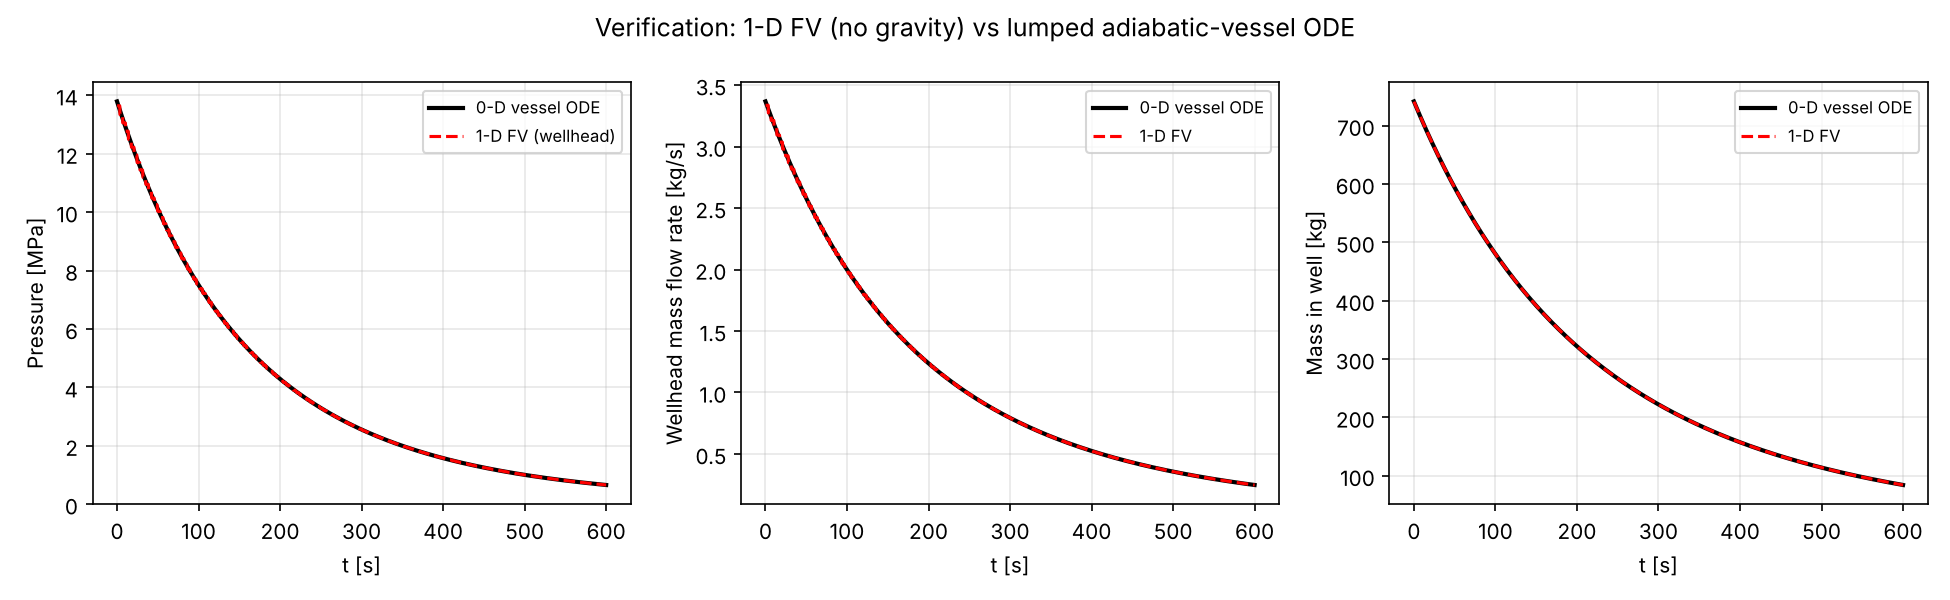
\includegraphics[width=\textwidth]{blowdown_vs_vessel_ode.png}
\caption{Verification against the lumped adiabatic-vessel ODE (gravity
off): wellhead pressure, mass flow rate, and mass inventory.}
\label{fig:vessel}
\end{figure}

\subsection{Grid, time-step, and boundary sensitivity}

For the baseline case over the first \SI{60}{s}, the maximum relative
deviation of $\mdot(t)$ from an 800-cell reference is
\SI{2.6}{\percent} (100 cells), \SI{0.88}{\percent} (200), and
\SI{0.26}{\percent} (400); reducing the CFL number from 0.9 to 0.5 and
0.2 changes $\mdot(t)$ by at most \SI{0.6}{\percent} and
\SI{1.2}{\percent}, respectively. A choke-bore sweep from
1/4\,in to the open-pipe limit (\cref{fig:choke}) yields initial
mass flow rates scaling with throat area as expected
(\num{0.84}/\num{3.32}/\num{12.9}/\SI{46.6}{kg/s}, open pipe
\SI{143}{kg/s}), monotonic throughout, stable in the pipe-choked limit,
and conservative to machine precision in every case.

\begin{figure}[htb]
\centering
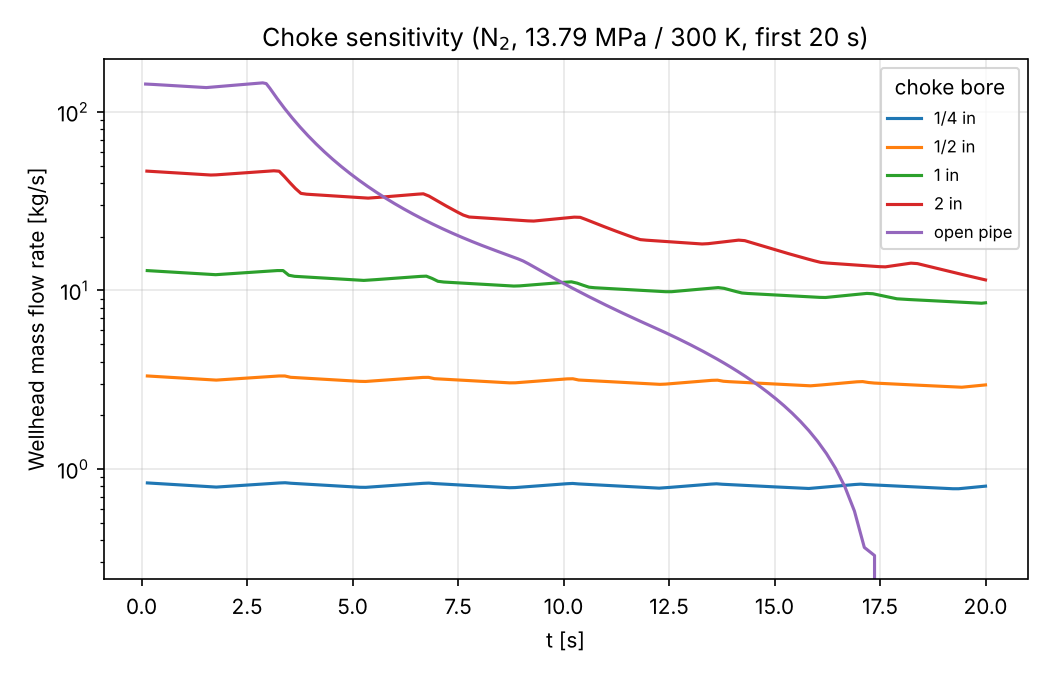
\includegraphics[width=0.72\textwidth]{blowdown_choke_sweep.png}
\caption{Sensitivity of the wellhead mass flow rate to the choke bore,
including the open-pipe limit.}
\label{fig:choke}
\end{figure}

%=============================================================
\section{Baseline results: adiabatic nitrogen blowdown}
%=============================================================
\label{sec:results}

\subsection{Wave propagation}

\Cref{fig:xt} presents the distance--time diagram of the pressure
perturbation $p - p_{\mathrm{init}}(z)$ during the first \SI{8}{s}, for a
run initialized in isothermal hydrostatic equilibrium so that the
valve-opening wave is the only transient (a uniform initial column
superposes a gravitational settling wave of comparable amplitude).
Opening the choke launches an expansion wave that descends the well at
the sound speed, reaching the bottom at $t = L/a_0 \approx \SI{1.7}{s}$,
reflecting, and returning to the wellhead at $2L/a_0 \approx \SI{3.4}{s}$;
since the choke passes only a small fraction of the sonic pipe flux, the
wellhead acts as a nearly closed end and the wave re-reflects as an
expansion, producing the staircase depressurization of period $2L/a_0$
with steps of $\mathcal{O}(\SI{130}{\kilo\pascal})$ visible in the
figure. Animations of the full field evolution accompany this document.
The initial expansion is weak relative to the inventory pressure
($\rho a\,\Delta u \sim \SI{1.5e5}{Pa}$ against \SI{13.79}{MPa}), and
the subsequent discharge is quasi-static --- consistent with the
lumped-vessel agreement above. Larger chokes proportionally strengthen
the initial wave.

\begin{figure}[htb]
\centering
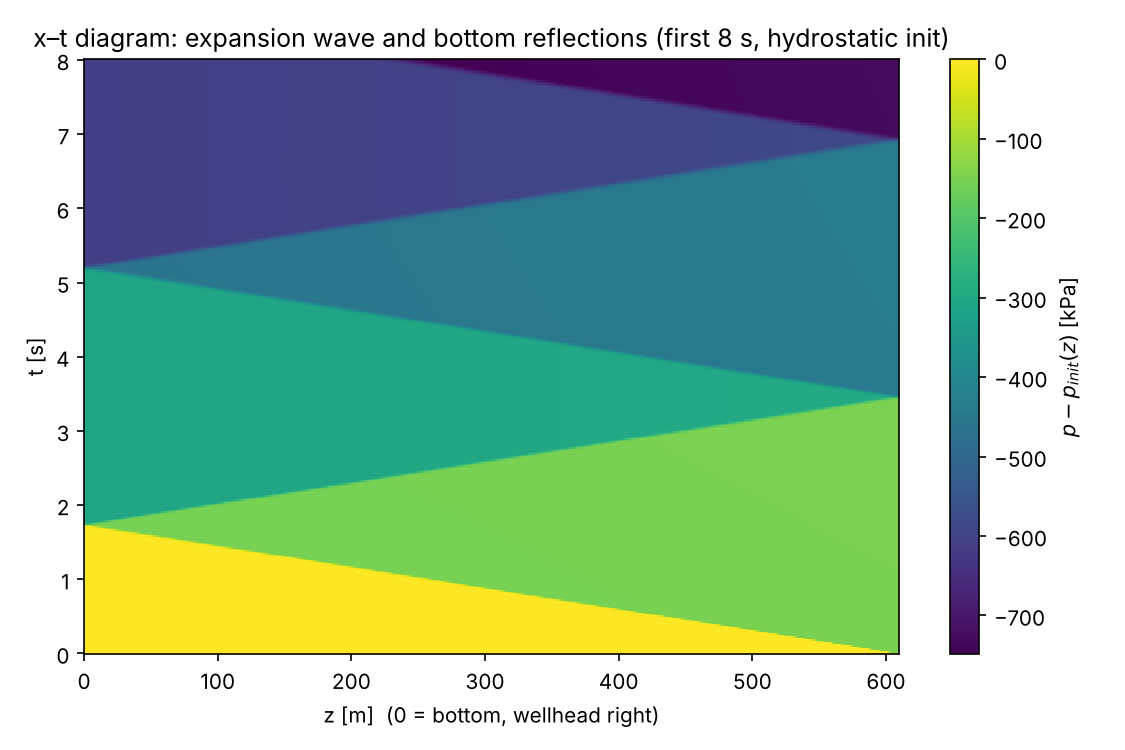
\includegraphics[width=0.8\textwidth]{blowdown_xt.png}
\caption{Distance--time ($x$--$t$) diagram of the pressure perturbation
$p - p_{\mathrm{init}}(z)$ during the first \SI{8}{s} after valve
opening (hydrostatic initialization): descending expansion wave, bottom
reflection, and staircase reverberation of period $2L/a_0$.}
\label{fig:xt}
\end{figure}

\subsection{Depressurization and cooling}

\Cref{fig:profiles,fig:histories} show the field profiles and wellhead
histories over \SI{600}{s}. The column depressurizes nearly uniformly
(mild top-to-bottom gradient sustained by the discharge plus the
hydrostatic head), the velocity profile is linear in $z$ --- the
signature of spatially uniform expansion --- with superposed decaying
acoustic oscillations, and the discharge remains choked for the entire
interval shown. Expansion work cools the inventory continuously; by
$t = \SI{600}{s}$ the wellhead fluid reaches \SI{127}{K}, i.e.\
essentially the critical temperature of nitrogen (\SI{126.2}{K}).

Two implications follow. First, the ideal-gas closure is increasingly
strained precisely where the blowdown terminates, quantifying the need
for the real-fluid property stage. Second, CO$_2$ under comparable
conditions would intersect its saturation locus far earlier in the
transient, so phase appearance is an expected feature, not an edge case,
of the CO$_2$ extension. In physical wells, heat ingress from the
completion and formation partially offsets this cooling, which is the
motivation for the conjugate thermal model of the next phase; a
prescribed-wall-temperature benchmark (Dittus--Boelter coupling,
$T_w = \SI{300}{K}$) indicates the magnitude of that offset.

\begin{figure}[htb]
\centering
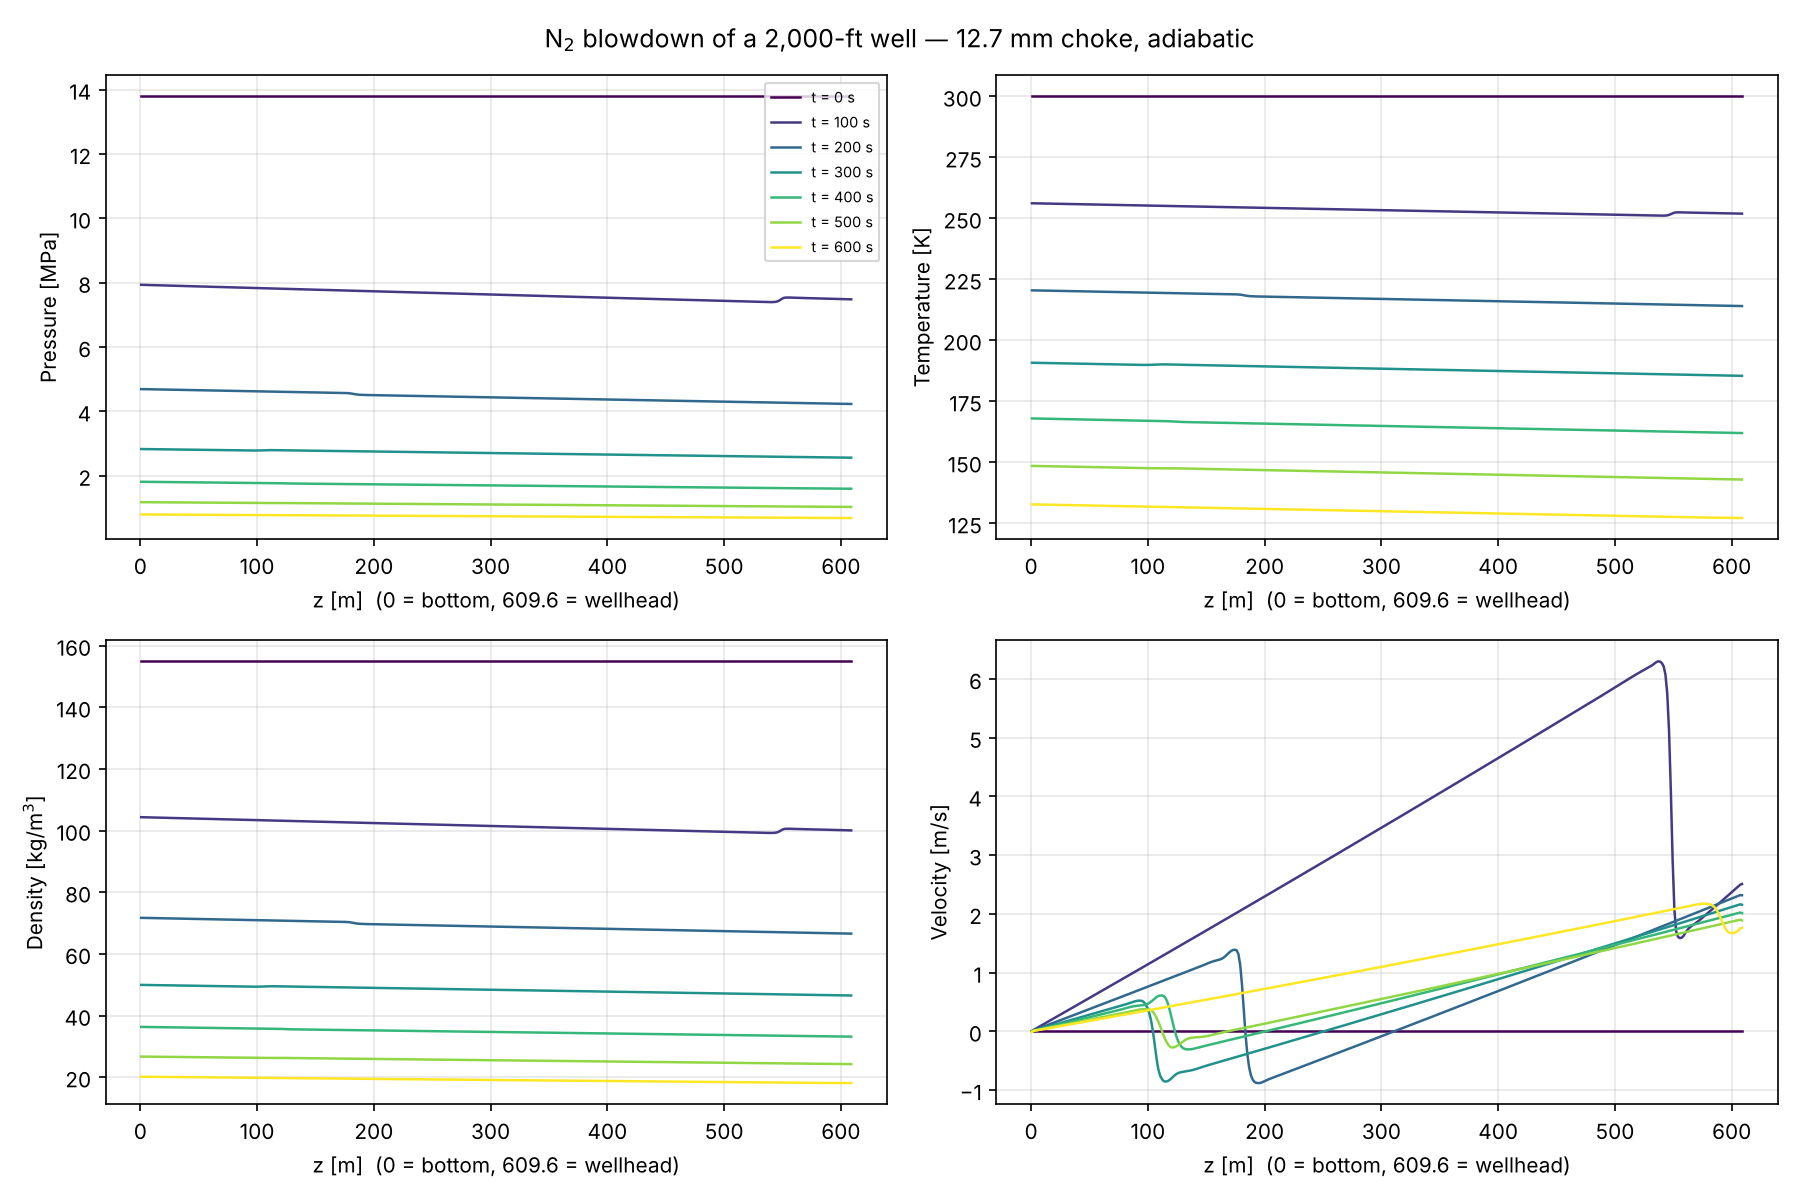
\includegraphics[width=\textwidth]{blowdown_profiles.png}
\caption{Axial profiles of pressure, temperature, density, and velocity
at \SI{100}{s} intervals during the baseline blowdown.}
\label{fig:profiles}
\end{figure}

\begin{figure}[htb]
\centering
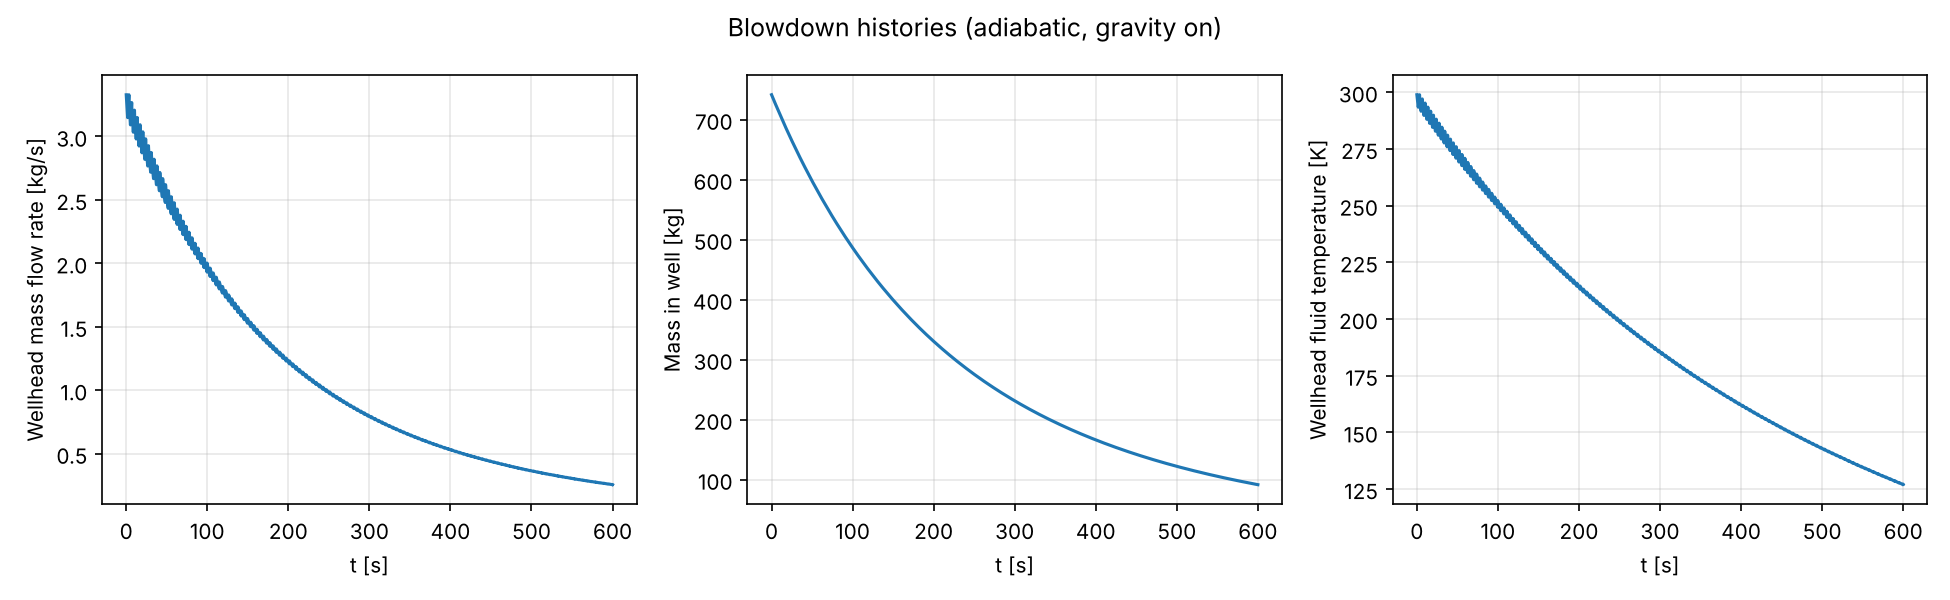
\includegraphics[width=\textwidth]{blowdown_histories.png}
\caption{Wellhead mass flow rate, mass inventory, and wellhead fluid
temperature during the baseline blowdown.}
\label{fig:histories}
\end{figure}

%=============================================================
\section{Conclusions and outlook}
%=============================================================
\label{sec:outlook}

A conservative Godunov/HLLC finite-volume model of vertical-well blowdown
has been implemented and verified for the adiabatic, ideal-gas stage:
discrete mass and total-plus-potential energy budgets close to machine
precision; the quasi-static limit reproduces the lumped-vessel solution
to better than \SI{1}{\percent}; and the characteristic-coupled choke
boundary condition behaves consistently from the choked regime through
valve closure, including the open-pipe limit. The baseline nitrogen case
exhibits the expected physics: a weak descending expansion wave and
reverberation, quasi-static discharge, and strong expansion cooling that
reaches the nitrogen critical temperature at the end of the transient.

The next stages, in order of priority: (i)~real-fluid CO$_2$
thermodynamics behind the existing property interface (single-phase
gaseous, then dense/transcritical), for which the end-of-blowdown
temperatures computed here already demonstrate the inadequacy of the
ideal-gas closure; (ii)~conjugate transient heat transfer, coupling the
wellbore energy equation to radial conduction through completion layers
and formation; and (iii)~phase appearance and two-phase CO$_2$ flow,
building on the two-phase benchmark heritage of the framework.

\section*{Code and data availability}
The implementation, verification scripts, and notebooks are maintained at
\url{https://github.com/JaderBarbosaLSU/hyperco2-wellbore}.

\bibliographystyle{plainnat}
\bibliography{references}

\end{document}
